\Question{Decision Trees Potpourri}

For the first two parts, we will consider a tree of depth 1 as shown in the diagram below. 

\begin{center}
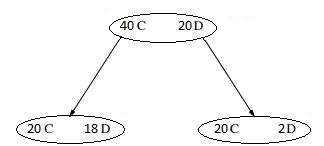
\includegraphics[width=3in]{src/problems/decision_tree/DecisionTree.jpg}
\end{center}

\begin{Parts}

\Part What is the entropy of the root node? Note, we use the base 2 log to calculate entropy.


\begin{solution}

$ H(X) = -\frac{40}{60}\log\frac{40}{60} - \frac{20}{60}\log\frac{20}{60} = 0.918 $

\end{solution}

\Part What is the information gain from splitting into the left and right nodes shown above?

\begin{solution}

$ H(X_L) = -\frac{20}{38}\log\frac{20}{38} - \frac{18}{38}\log\frac{18}{38} $ \\
$ H(X_R) = -\frac{20}{22}\log\frac{20}{22} - \frac{2}{22}\log\frac{2}{22} $ \\
$ H(X_\text{split}) = \frac{38}{60}H(X_L) + \frac{22}{60}H(X_R) $ \\
$ I = H(X) - H(X_\text{split}) = 0.125 $\\
\end{solution}

For the next few parts, consider constructing a depth-2 decision tree on data with $f$ features, where each feature is real-valued and each label takes one of $l$ possible values. Each split in the decision tree is chosen to greedily maximize information gain. Ties between different split that equally maximize information gain are chosen arbitrarily.

\Part
Prove or give a counter-example: For every value of $l > 3$, there exists some probability distribution on $n$ training points such that its entropy is less than -1.

\begin{solution}
  False. The entropy is always non-negative since $-p \log p$ is non-negative for $p \in [0, 1]$.
\end{solution}

\Part Give an example of a dataset with $f=4$ and $l=2$ where same feature is split on twice.

\begin{solution}
  If the labels are + and -, and our training points [represented as (x1, x2, x3, label) tuples] are: \\

  (1, 0, 0, +), (2, 0, 0, -) (3, 0, 0, +)

Then we split on the first feature twice.
\end{solution}


\Part Prove or give a counter-example: The information gain at the root is at least as much as the information gain at any other node.

\begin{solution}
False. As a counterexample, consider the following "XOR" dataset, where "X" labels are found in quadrants 2 and 4, but "O" labels are found in quadrants 1 and 3.

No matter which split is chosen first, we will have zero information gain. But is possible to
gain information on the second splits.
\end{solution}

Now we will consider a more general decision tree. 

\Part We are creating a spam filter using a decision tree, and our tree has 99\% training accuracy on a balanced dataset. However, our validation accuracy is only 65\%. Which of the following are valid ways to improve our test performance?


Reduce the depth/height of our tree\\
Increase the depth/height of our tree\\
Upon reaching some threshold in training accuracy, we stop growing our tree\\
Train on a subset of our training data\\

\begin{solution}
The fact that we do much better on our training set than our validation set is a symptom of us overfitting to the training data. To reduce overfitting, reducing the depth and setting a threshold are valid options. Reducing the depth and prematurely stopping tree growth are both ways to prevent our tree from fitting perfectly to the training data. Training only on a subset of the training data is essentially throwing away information, and although it may help sometimes, it is usually a good idea to look at other ways to reduce overfitting. 
\end{solution}

\end{Parts}

\newpage
